\section{Partitore resistivo}
In questa parte di esperienza abbiamo studiato la seguente configurazione:

\begin{figure}[H]
    \centering
    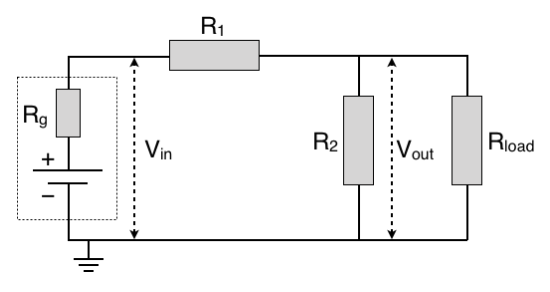
\includegraphics[scale=1]{Immagini/PartResist.PNG}
    \label{fig:my_label}
\end{figure}

nella quale con $R_{load}$ indichiamo il partitore resistivo, componente di circuito di cui è possibile scegliere la resistenza attraverso interruttori.
Abbiamo studiato la configurazione sotto la condizione in cui $V_{out}$ = 0.5$V_{in}$.
Attraverso considerazioni sulle resistenze equivalenti e sulla confrontabilità tra la resistenza del partitore e quelle note, siamo arrivati alla conclusione per la quale, al fine di avere una configurazione con la condizione sopra citata, era necessario che $R_{1}$ ed $R_{2}$ fossero uguali e che $R_{load}$ fosse mandata a infinito. Nella pratica, questa procedura è stata compiuta aumentando sempre più la resistenza del partitore.

\begin{equation}
R_{eq} = \frac{R_{2}R_{load}}{R_{2}+R_{load}} \hspace{73 pt} R_{tot} = R_{1}+\frac{R_{2}R_{load}}{R_{2}+R_{load}}
\end{equation}
\begin{equation}
\label{eq: 5}
V_{in} = R_{tot}I \hspace{73 pt} V_{out} = R_{eq}I = V_{in}\frac{R_{eq}}{R_{1}+R_{eq}}  
\end{equation}
\noindent
Dalla equazione \ref{eq: 5} è evidente che, nel caso in cui  $R_{load}\to \infty$ e $V_{out}$ = 0.5$V_{in}$, si ottiene \begin{equation}
\frac{1}{2} = \frac{R_{2}}{R_{1}+R_{2}} \hspace{20 pt} \text{per cui} \hspace{20 pt} R_{1} = R_{2}
\end{equation}

Abbiamo confermato queste osservazioni sperimentalmente (utilizzando come resistenze $R_{1} = R_{2} = 150k\Omega)$, come risulta visibile dal grafico:

\begin{figure}[H]
    \centering
    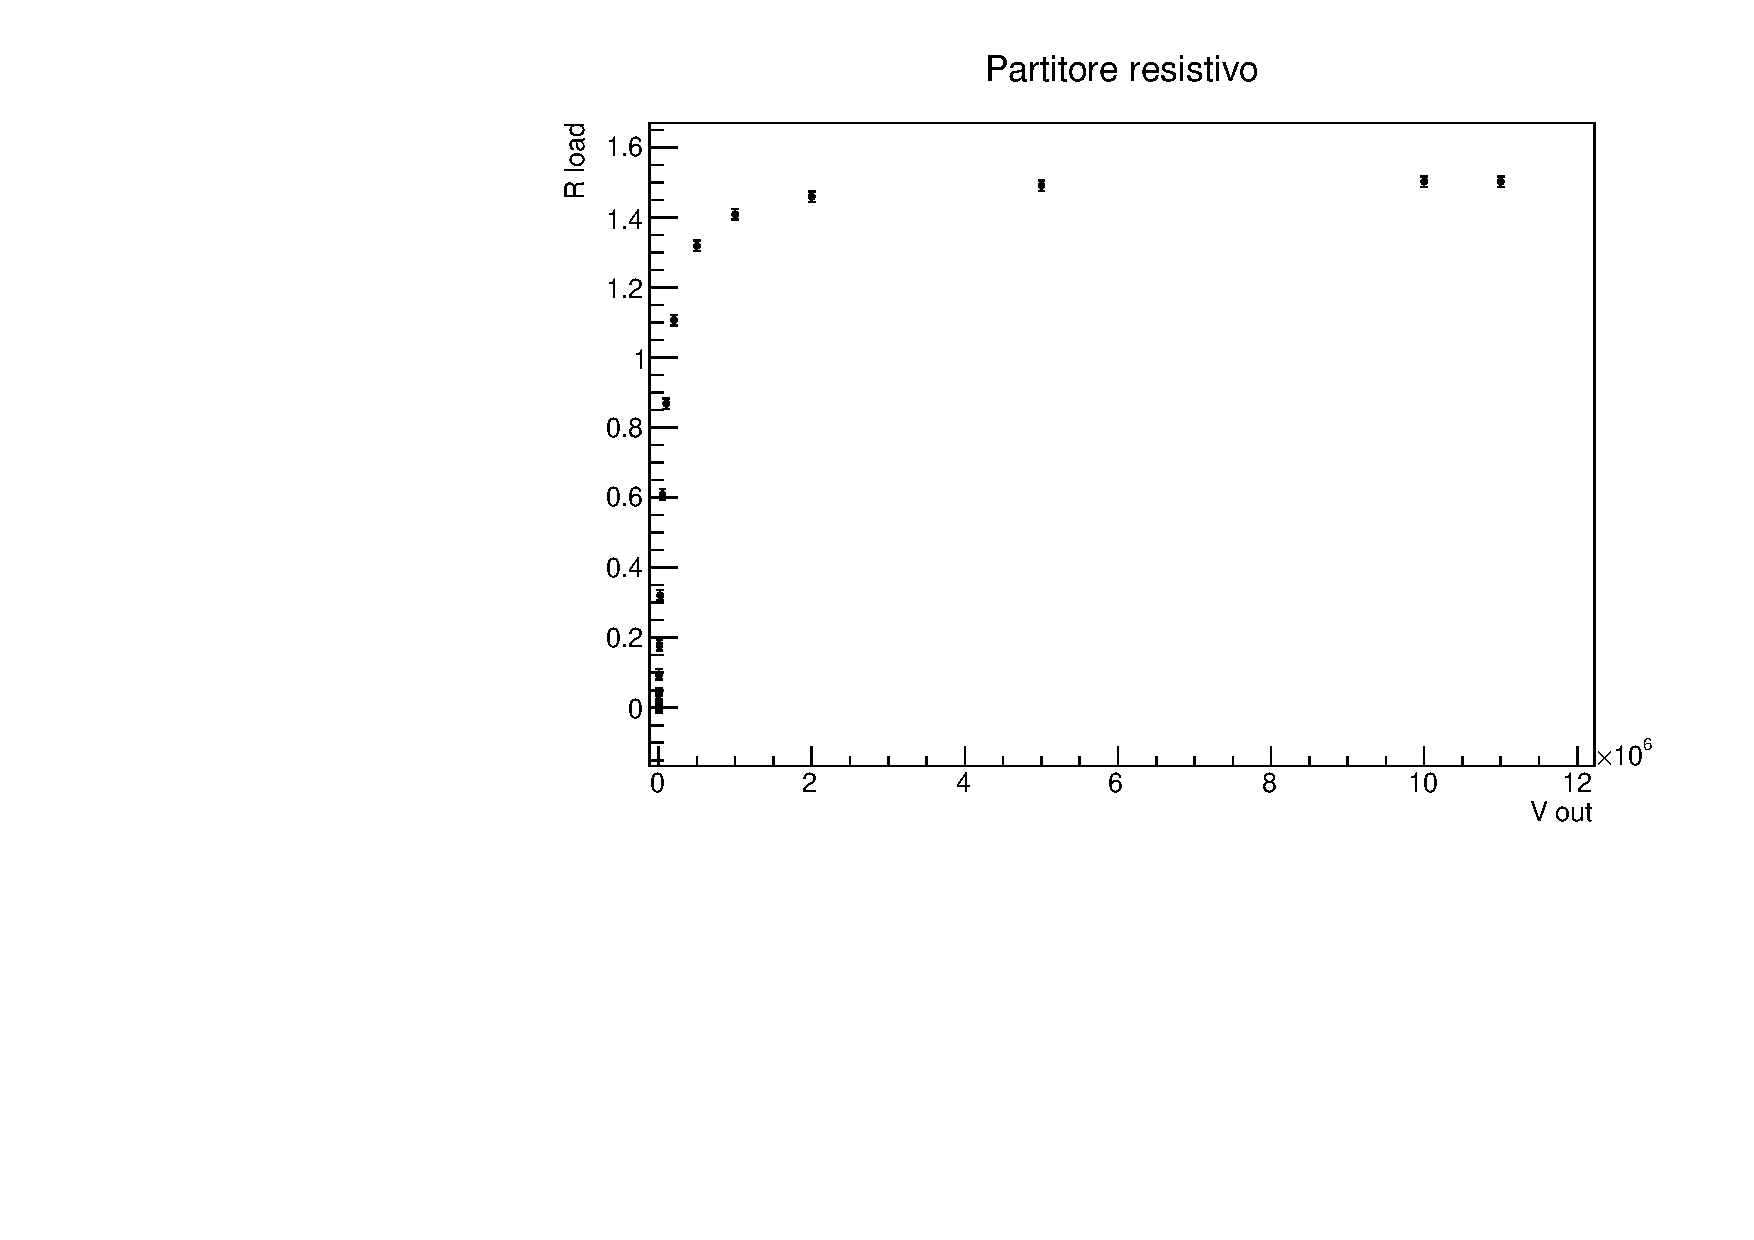
\includegraphics[scale=.6]{partitore resistivo.pdf}
    \caption{}
    \label{fig: partitore resistivo}
\end{figure}